\documentclass[tikz,border=3pt]{standalone}
\usepackage{tikz}
\begin{document}
% \begin{tikzpicture}[x=1cm,y=1cm]
% % Execution environments (top row)
% \draw[fill=blue!10] (0.1,5.25) rectangle (1.8,5.65) node[pos=.5]{\scriptsize HPC};
% \draw[fill=blue!10] (1.8,5.25) rectangle (3.6,5.65) node[pos=.5]{\scriptsize Cloud};
% \draw[fill=blue!10] (3.6,5.25) rectangle (5.4,5.65) node[pos=.5]{\scriptsize Edge};
% \draw[fill=blue!10] (5.4,5.25) rectangle (7.1,5.65) node[pos=.5]{\scriptsize Devices};
% \node[font=\scriptsize\itshape] at (3.6,5.9) {Execution environments};

% % L1-L6 as 6 vertical columns (boxes and text rotated 90°)
% % Column width = 7.0cm / 6 = 1.1667cm each; height = 2.30 to 4.95
% \draw[fill=gray!10] (0.10,2.30) rectangle (1.27,4.95);
% \node[rotate=90, font=\scriptsize] at (0.683,3.625)
%   {\shortstack{\textbf{L1}\\[2pt]Hardware\\(RoT, PhySec)}};

% \draw[fill=gray!10] (1.27,2.30) rectangle (2.43,4.95);
% \node[rotate=90, font=\scriptsize] at (1.850,3.625)
%   {\shortstack{\textbf{L2}\\[2pt]Software\\(OS, MW, OTA)}};

% \draw[fill=gray!10] (2.43,2.30) rectangle (3.60,4.95);
% \node[rotate=90, font=\scriptsize] at (3.017,3.625)
%   {\shortstack{\textbf{L3}\\[2pt]Application\\(Workloads, APIs)}};

% \draw[fill=gray!10] (3.60,2.30) rectangle (4.77,4.95);
% \node[rotate=90, font=\scriptsize] at (4.183,3.625)
%   {\shortstack{\textbf{L4}\\[2pt]User \& Orch.\\(ZT, IAM, PAM)}};

% \draw[fill=gray!10] (4.77,2.30) rectangle (5.93,4.95);
% \node[rotate=90, font=\scriptsize] at (5.350,3.625)
%   {\shortstack{\textbf{L5}\\[2pt]Data-Centric\\(PQC, TEE, QKD, SMPC)}};

% \draw[fill=gray!10] (5.93,2.30) rectangle (7.10,4.95);
% \node[rotate=90, font=\scriptsize] at (6.517,3.625)
%   {\shortstack{\textbf{L6}\\[2pt]Network \&\\Perimeter}};

% % Cross-layers
% \draw[fill=orange!15,dashed] (0.1,1.75) rectangle (7.1,2.10) node[pos=.5]{\scriptsize CL1: Cyber-Resilient SW/AI Lifecycle};
% \draw[fill=orange!15,dashed] (0.1,1.35) rectangle (7.1,1.70) node[pos=.5]{\scriptsize CL2: Dynamic Risk and SecOps};
% \draw[fill=orange!15,dashed] (0.1,0.95) rectangle (7.1,1.30) node[pos=.5]{\scriptsize CL3: Interoperability (Simpl, CAMARA, MIMs)};
% \draw[fill=orange!15,dashed] (0.1,0.55) rectangle (7.1,0.90) node[pos=.5]{\scriptsize CL4: Compliance-by-Design and Assurance};
% % Figure label
% \node[font=\small\itshape, anchor=north] at (3.6,0.3)
%   {Fig.~1: Layered security model for the Cloud--Edge--IoT continuum.};
% \end{tikzpicture}

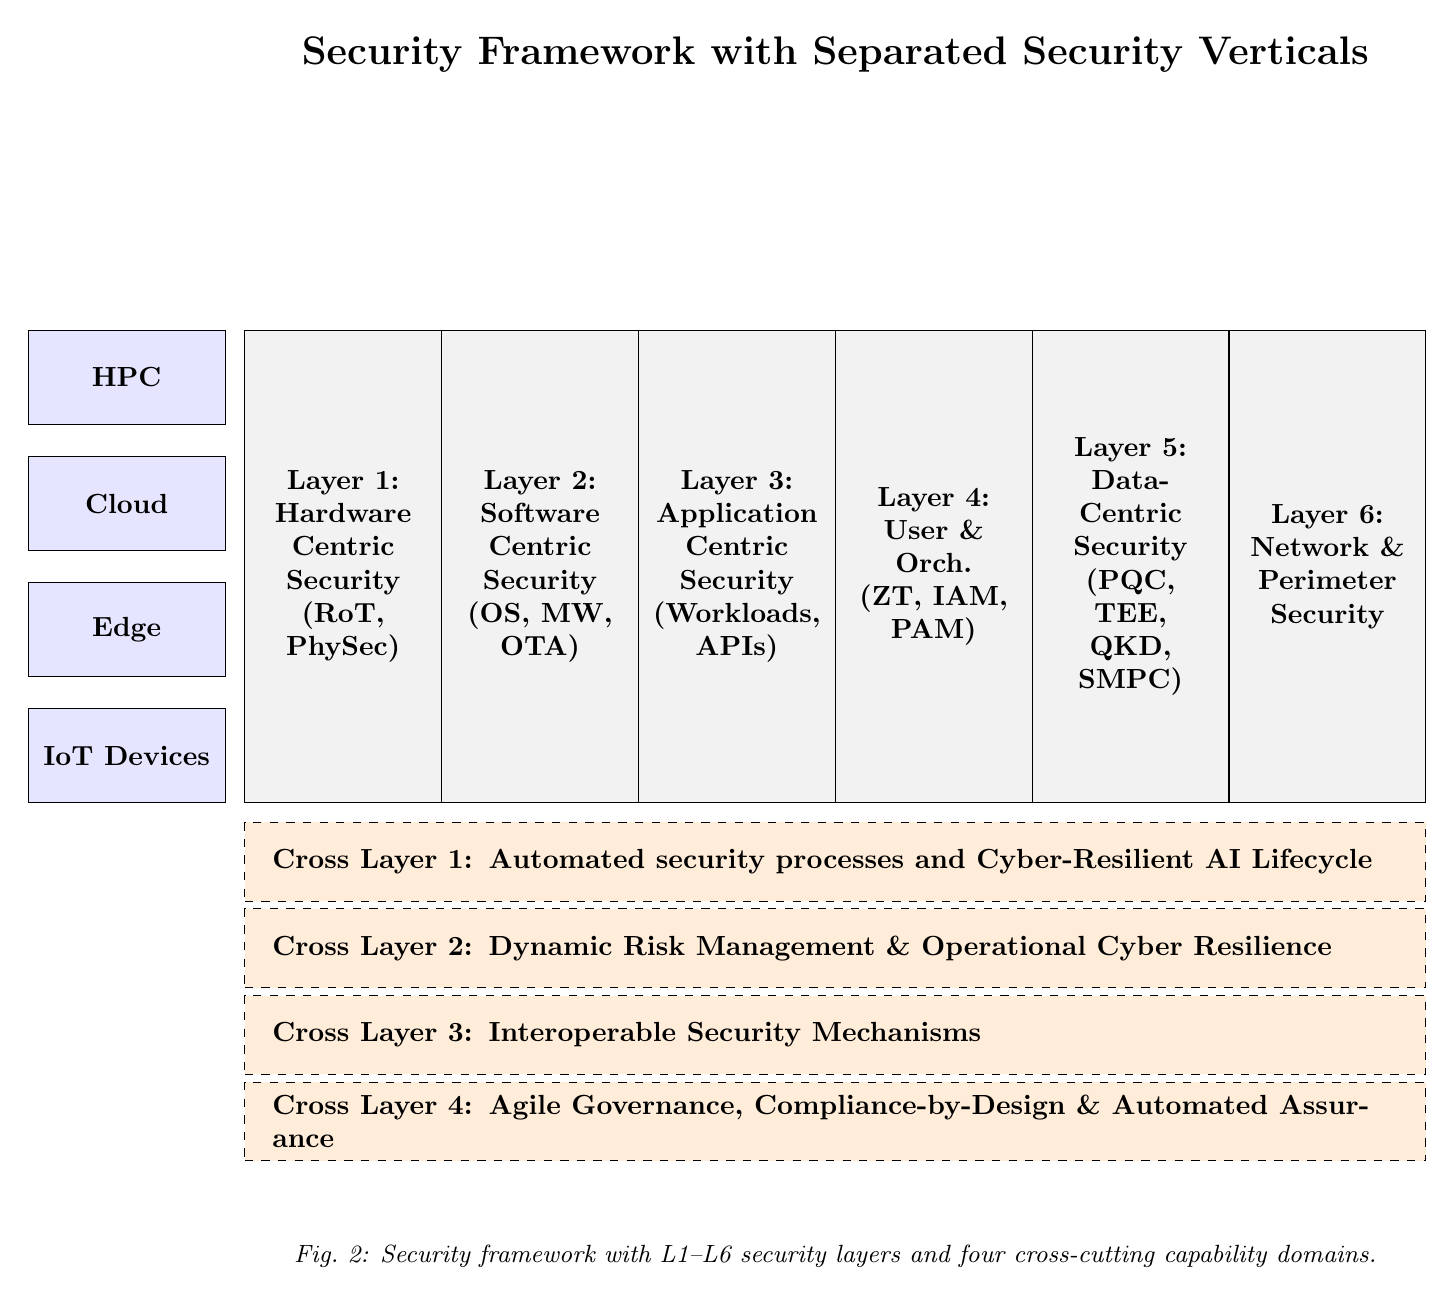
\begin{tikzpicture}[every node/.style={font=\small}]

    % Styles — matching figure 1 colours
    \tikzstyle{arch_col} = [fill=gray!10, draw=black, text=black, font=\bfseries,
        minimum width=2.5cm, minimum height=6cm, align=center, text width=2.2cm]
    \tikzstyle{env_box} = [fill=blue!10, draw=black, text=black, font=\bfseries,
        minimum width=2.5cm, minimum height=1.2cm, align=center]
    \tikzstyle{vertical_box} = [fill=orange!15, draw=black, dashed, text=black,
        font=\bfseries, minimum width=15.0cm, minimum height=1cm,
        align=left, text width=14.3cm]

    % Column X positions: 6 columns × 2.5cm width, adjacent (spacing = 2.5cm)
    % Total span: 15cm, centred → from -7.5 to 7.5
    \def\colone{-6.25}
    \def\coltwo{-3.75}
    \def\colthree{-1.25}
    \def\colfour{1.25}
    \def\colfive{3.75}
    \def\colsix{6.25}

    % Environment boxes (left) — blue!10 as in figure 1
    \node[env_box] at (-9, 2.4) {HPC};
    \node[env_box] at (-9, 0.8) {Cloud};
    \node[env_box] at (-9, -0.8) {Edge};
    \node[env_box] at (-9, -2.4) {IoT Devices};

    % Main architecture columns L1–L6 — gray!10 as in figure 1
    \node[arch_col] at (\colone,  0) {Layer 1:\\ Hardware\\ Centric Security\\ (RoT, PhySec)};
    \node[arch_col] at (\coltwo,  0) {Layer 2:\\ Software\\ Centric Security\\ (OS, MW, OTA)};
    \node[arch_col] at (\colthree,0) {Layer 3:\\ Application\\ Centric Security\\ (Workloads,\\ APIs)};
    \node[arch_col] at (\colfour, 0) {Layer 4:\\ User \& Orch.\\ (ZT, IAM, PAM)};
    \node[arch_col] at (\colfive, 0) {Layer 5:\\ Data-Centric\\ Security\\ (PQC, TEE,\\ QKD, SMPC)};
    \node[arch_col] at (\colsix,  0) {Layer 6:\\ Network \&\\ Perimeter\\ Security};

    % Cross-layer vertical boxes — orange!15 dashed as in figure 1 (adjacent, 1.1cm spacing)
    \node[vertical_box] at (0, -3.75) {Cross Layer 1: Automated security processes and Cyber-Resilient AI Lifecycle};
    \node[vertical_box] at (0, -4.85) {Cross Layer 2: Dynamic Risk Management \& Operational Cyber Resilience};
    \node[vertical_box] at (0, -5.95) {Cross Layer 3: Interoperable Security Mechanisms};
    \node[vertical_box] at (0, -7.05) {Cross Layer 4: Agile Governance, Compliance-by-Design \& Automated Assurance};

    % Title
    \node[font=\Large\bfseries, anchor=center] at (0, 6.5) {Security Framework with Separated Security Verticals};

    % Figure label
    \node[font=\small\itshape, anchor=north] at (0, -8.5)
      {Fig.~2: Security framework with L1--L6 security layers and four cross-cutting capability domains.};

\end{tikzpicture}
\end{document}
